% ==========================================================
% TEMPLATE PROFISSIONAL IESB - RELATÓRIO TÉCNICO
% Curso: Ciência de Dados e Inteligência Artificial
% Curso: Mestrado em Gestão Estratégica de Organizaçoes (MGEO) 
% Formato ABNT (abntex2)
% ==========================================================

\documentclass[
    12pt,
    oneside,
    a4paper,
    chapter=TITLE,
    section=TITLE
]{abntex2}

% ----------------------------------------------------------
% PACOTES
% ----------------------------------------------------------
\usepackage[T1]{fontenc}
\usepackage[utf8]{inputenc}
\usepackage[brazil]{babel}
\usepackage{lmodern}
\usepackage{graphicx}
\usepackage{float}
\usepackage{microtype}
\usepackage{indentfirst}
\usepackage{hyperref}
\usepackage{xcolor}
\usepackage{listings}
\usepackage{fancyhdr}

% ----------------------------------------------------------
% CITAÇÕES E REFERÊNCIAS ABNT
% ----------------------------------------------------------
\usepackage[alf]{abntex2cite}

% ----------------------------------------------------------
% CORES
% ----------------------------------------------------------
\definecolor{iesbRed}{RGB}{170,0,0}
\definecolor{codegray}{RGB}{245,245,245}

% ----------------------------------------------------------
% CONFIGURAÇÃO DE CÓDIGOS
% ----------------------------------------------------------
\lstset{
    backgroundcolor=\color{codegray},
    basicstyle=\ttfamily\small,
    frame=single,
    breaklines=true,
    numbers=left,
    numberstyle=\tiny
}

% ----------------------------------------------------------
% CAMPOS INSTITUCIONAIS (EDITAR AQUI)
% ----------------------------------------------------------
\newcommand{\iesbcurso}{Graduação em Ciência de Dados e Inteligência Artificial}
\newcommand{\iesbdisciplina}{CIA014 - Análise Exploratória de Dados e Visualização}
\newcommand{\iesbsemestre}{2026/1}
\newcommand{\iesbautor}{Sérgio da Costa Côrtes}
\newcommand{\iesbtitulo}{--- Título do trabalho ---}

% ----------------------------------------------------------
% DADOS ABNTEX
% ----------------------------------------------------------
\titulo{\iesbtitulo}
\autor{\iesbautor}
\local{Brasília -- DF}
\data{2026}

\instituicao{
Centro Universitário IESB\\
Graduação em Ciência de Dados e Inteligência Artificial
}

\tipotrabalho{Relatório Técnico}

% ----------------------------------------------------------
% LAYOUT INSTITUCIONAL (CABEÇALHO/RODAPÉ)
% ----------------------------------------------------------
\pagestyle{fancy}
\fancyhf{}

\fancyhead[L]{\footnotesize IESB • \iesbcurso}
\fancyhead[R]{\footnotesize \thepage}

\fancyfoot[L]{\footnotesize \iesbdisciplina\ • \iesbsemestre}
\fancyfoot[R]{\footnotesize \iesbautor}

\renewcommand{\headrulewidth}{0.3pt}
\renewcommand{\footrulewidth}{0pt}
\setlength{\headheight}{14.5pt}

% ==========================================================
% INÍCIO DO DOCUMENTO
% ==========================================================
\begin{document}

% ----------------------------------------------------------
% PRÉ-TEXTUAL SEM NUMERAÇÃO VISÍVEL (ABNT)
% ----------------------------------------------------------
\pagenumbering{arabic}
\pagestyle{empty}

% ==========================================================
% CAPA
% ==========================================================
\begin{capa}
\centering


\includegraphics[width=0.22\textwidth]{Figuras/IESB_logo.png}

\vspace{1.5cm}

{\Large\bfseries CENTRO UNIVERSITÁRIO IESB}

\vspace{0.5cm}

{\large Graduação em Ciência de Dados e Inteligência Artificial}

\vfill

{\color{iesbRed}\bfseries\Huge RELATÓRIO TÉCNICO}

\vspace{1cm}

{\Large \iesbtitulo}

\vfill

\iesbautor

\vfill

Brasília -- DF\\
2026

\end{capa}

% ----------------------------------------------------------
% FOLHA DE ROSTO
% ----------------------------------------------------------
\folhaderosto*

% ----------------------------------------------------------
% RESUMO
% ----------------------------------------------------------
\begin{resumo}

Este relatório técnico apresenta o desenvolvimento de atividades relacionadas à Ciência de Dados e Inteligência Artificial, contemplando coleta, tratamento, modelagem e análise de dados, bem como interpretação dos resultados obtidos.

\vspace{\onelineskip}

\noindent
\textbf{Palavras-chave}: ciência de dados. inteligência artificial. machine learning. análise de dados.

\end{resumo}

% ----------------------------------------------------------
% SUMÁRIO E LISTAS
% ----------------------------------------------------------
\tableofcontents*
\listoffigures*
\listoftables*

% ==========================================================
% INÍCIO DO TEXTO (NUMERAÇÃO ATIVA)
% ==========================================================
\cleardoublepage
\pagestyle{fancy}
\textual

% ----------------------------------------------------------
\chapter{Introdução}

Contextualização do problema, objetivos e justificativa do trabalho.

Para citar uma fonte bibliográfica use \cite{goodfellow2016}.

Para outra citação \cite{ibge2025}

% ----------------------------------------------------------
\chapter{Fundamentação Teórica}

Base conceitual utilizada no projeto.

% ----------------------------------------------------------
\chapter{Metodologia}

Descrição dos dados, ferramentas e métodos utilizados.

\section{Ambiente Computacional}

Exemplo: Python, SAS Viya, PostgreSQL, etc.

% ----------------------------------------------------------
\section{Código Python}

\begin{lstlisting}[language=Python,caption={Exemplo em Python}]
import pandas as pd

df = pd.read_csv("dados.csv")
print(df.head())
\end{lstlisting}

% ----------------------------------------------------------
\section{Código SAS}

\begin{lstlisting}[caption={Exemplo em SAS}]
proc means data=meusdados;
run;
\end{lstlisting}

% ----------------------------------------------------------
\chapter{Resultados e Discussão}

% Figuras sem margem

\begin{figure}[H]
\centering
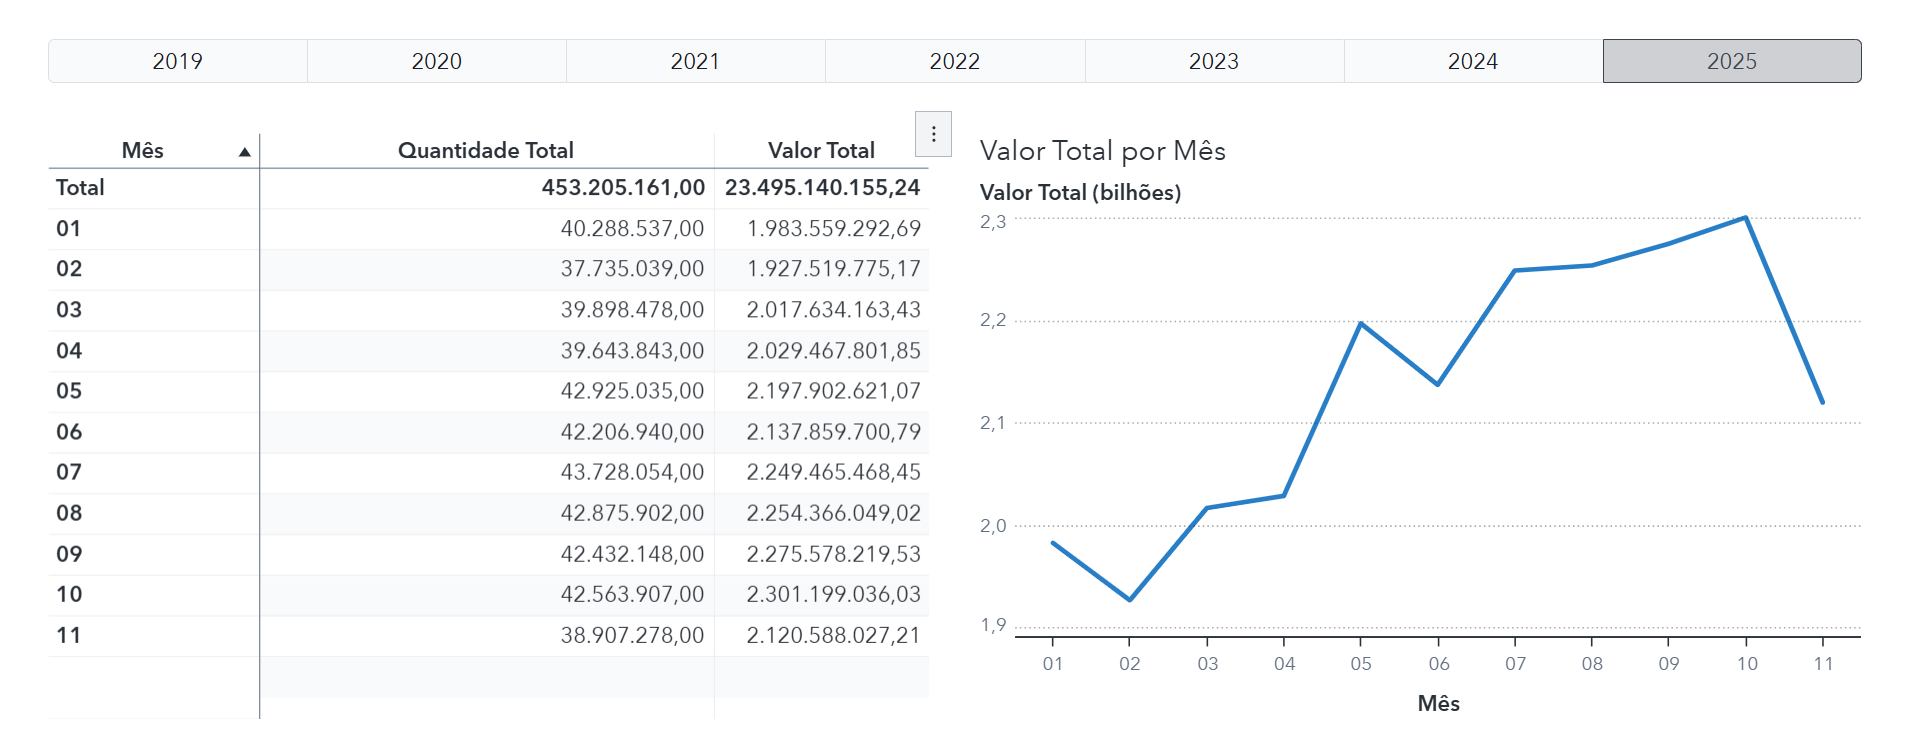
\includegraphics[width=0.7\textwidth]{Figuras/SUS_AIH_Ano_Mes.png}
\caption{Figura sem moldura ajustada}
\label{fig:resultado}
\end{figure}

% Figuras com margem

\begin{figure}[H]
\centering
\setlength{\fboxrule}{1pt}
\setlength{\fboxsep}{5pt}
\fbox{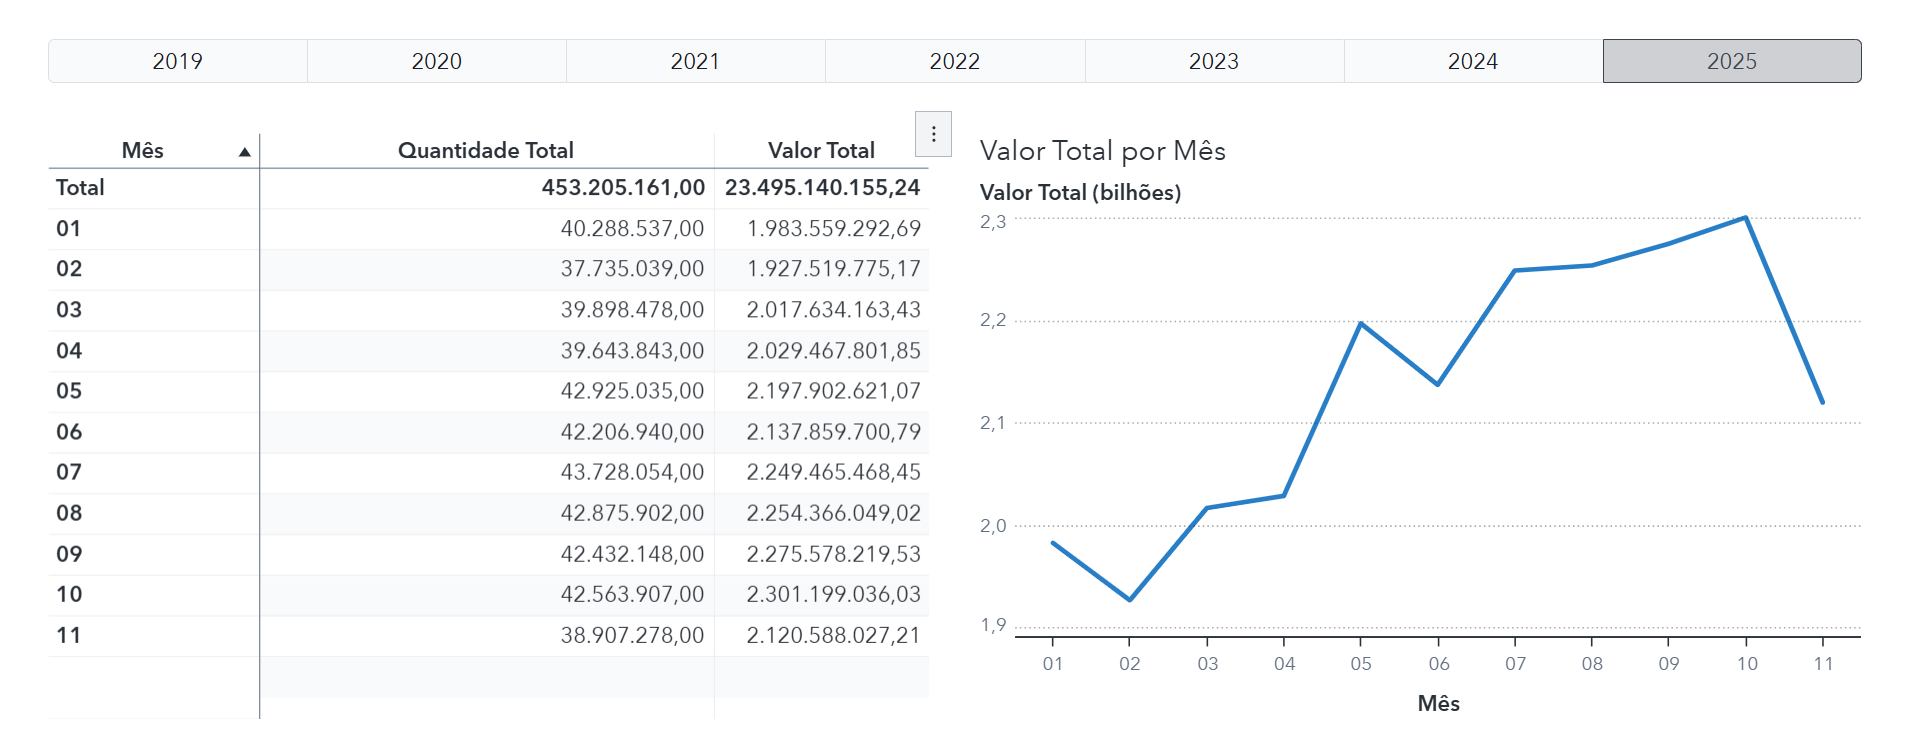
\includegraphics[width=0.7\textwidth]{Figuras/SUS_AIH_Ano_Mes.png}}
\caption{Figura com moldura ajustada}
\label{fig:resultado2}
\end{figure}


% ----------------------------------------------------------
\chapter{Conclusão}

Principais conclusões e trabalhos futuros.

% ==========================================================
% REFERÊNCIAS ABNT
% ==========================================================
\postextual
\bibliography{referencias}

\end{document}